\chapter{Fuzzing}
\label{cha:3:fuzzing}
\label{fuzzing:intro}
The rise of fuzzing came with Miller giving his classroom assignment \cite{21FuzzingAssignment} in 1988 to his computer science students to test Unix utilities with randomly generated inputs with the goal to break the utilities. Two years later in December he wrote a paper \cite{4originalFuzzingUnixUtils} about the remarkable results that more than 24\% to 33\% of the programs tested crashed.
In the last thirty years the technique of fuzzing has changed significantly and various innovations have come forward. In this chapter we will look at prevalent classifications made, what the fuzzer expects as input, what we can expect as output and we will look at the most popular fuzzers.

\section{Classifications}
\label{fuzzing:Classifications}
The three most popular classifications are: how does the fuzzer create input, how well is the input structured and does the fuzzer have knowledge of the program under test (PUT) \cite{30FuzzingHackartandscience, 12Fuzzingasurvey, 13manes2019survey}.

\subsection{Generation and mutation}
\label{fuzzing:generationMutation}
A fuzzer can construct inputs for a PUT in two ways, it can generate input itself or it can modify parts from an existing input, called seeds. While Generation is more common when it comes to smaller inputs, the opposite is true for larger inputs where modification has the upper hand. This is caused by the fact that generating semi-valid input becomes a lot harder the longer the input becomes. For example, generating the word "Fuzzing" by uniformly random sample of ASCII symbols, has a chance of one in $5*10^{14}$ of happening, making this technique infeasible when we want to generate bigger semi-valid inputs. With mutation we can start with larger and already valid input and then make modifications to create semi-valid inputs. With this last technique the diversity of the seeding inputs does become quite important. Ideally, we would have an unlimited diverse set of inputs, but that may not always be available. A workaround to this issue could be the paper by Alexandre Rebert et al. \cite{14rebert2014seedselecting} they propose that seed selection algorithms can improve results and compare random seed selection to the minimal subset of seeds with the highest code coverage among other algorithms. 

\subsection{Input structure}
\label{fuzzing:InputStructure}
%lexical, sementical, constraint or random
While we have discussed the bigger scope on how inputs are created, let us go into more detail; as we have seen before, fuzzing started with Miller's classroom assignment. This random generation of inputs falls under 'dumb' fuzzing due to only seeing the input as one long list of independent symbols with no knowledge of any input structure. This technique can be applied similarly to mutational fuzzing as well, compared to only adding symbols with generational fuzzing here we also remove or change randomly selected symbols. 
We can create three types of inputs: non-valid, semi-valid and valid inputs. With non-valid inputs we will almost be exclusively testing the lexical and syntactic stage of the PUT, which often comes down to just the parser. Either the input crashes the parser or it will be detected and the PUT will stop running. With semi-valid inputs we hope to be as close as possible to valid inputs in order to explore beyond the parser and to catch bugs deeper in the PUT. And finally, with valid input we are testing if the PUT behaves as expected and does not crash, although we cannot know which type a given input is before giving it to the PUT.
A smart fuzzer referrers to the fuzzing techniques which have knowledge about the structure inputs can or should have. This increases the chance of inputs passing the parser and being able to test the deeper parts of the PUT, this at the cost of needing an increased complex fuzzer. We can build a 'smart' fuzzer by adding knowledge about keywords (making it a lexical fuzzer) or by adding knowledge about syntax (for a syntactical fuzzer. The latter one can for example match all parentheses), while the former would be able to create correct keywords such as "continue" for example. Directed fuzz testing, where we guide the fuzzer on a specific code location via an explicit path, does fit in this category of a 'smart' fuzzer as well but it is not possible in a black box environment, more on that in the next section.

\subsection{Black, gray and white box fuzzing}
\label{fuzzing:BlackGrayWhiteFuzzing}
On top of adding knowledge of the inputs' structure to the fuzzer, we can also add knowledge of the program under tests' structure to the fuzzer. Which brings us to black, gray and white box fuzzing. With black box fuzzing the fuzzer does not have any knowledge about the inner working of the PUT and we treat the PUT as a literal black box. We provide input and we look at what the PUT provides as output. With this minimal information the fuzzer then tries to improve its input creation. 
Compared to black box fuzzing, gray box fuzzing usually comes with tools that give indirect information to the fuzzer. Tools like code coverage, timings, classes of errors as measurements are all used as feedback, but more measurements are possible. 
Lastly white box testing is the term used when the fuzzer has as much information available as possible. It will have access to the source code and can adjust their inputs to fuzz specific parts of the code. Directed fuzzing also falls under this term, here we guide the fuzzer to interesting locations for testing of specific parts of the PUT. White box fuzzing does have a higher computation cost due to having to reverse engineer the path to specific edge cases, meaning that it has a higher chance of finding more bugs per input but creating those inputs takes more time compared to black box fuzzing. 

The differentiation between black, gray and white box fuzzing is not clear cut, most people would agree that white box fuzzing has full knowledge about the PUT, including the source code, that gray box fuzzing has some knowledge about the PUT and that black box fuzzing has little to no knowledge about the PUT. Going into more detail could become controversial, all we can say is that it is no longer a black-and-white situation and that the lines have become fuzzy.

\section{Classifying popular fuzzers}
\label{fuzzing:OtherFuzzers}
Now that we know how we can classify fuzzers, let us look at some existing fuzzers to see how they work. For starters Miller's original work, which we discussed earlier, was a random generation based black box fuzzing. It started off as an assignment for his students to test the reliability of Unix utility programs by trying to break them using a fuzz generator, which was able to generate printable ASCII, non-printable ASCII, with or without null terminating characters of a random length. That resulted in a successful paper two years later \cite{4originalFuzzingUnixUtils}. His later work in 1995 on even more UNIX utilities, X-Windows servers \cite{26miller1995fuzzrevisited} in 1995, Windows NT 4.0 and Windows 2000 \cite{24MillerWindows} in 2000, MacOS \cite{25MillerOnMacOS} in 2006 and his recent revisit in 2020 on fuzzing \cite{3miller2020relevanceOfClasicalFuzzTesting} all fall in the same category of random generation based black box fuzzing. His papers showed that a significant portion of programs are able to be crashed with random inputs. Of the programs tested 15\% to 43\% of the Unix utilities crashed, 6\% of the open-source GNU utilities crashed, 26\% of X-Window applications crashed, 45\% of Windows NT 4.0 and Windows 2000 programs crashed and 16\% MacOS programs crashed.

A couple of years later, KLEE \cite{8KLEE} was developed by Cadar et al. KLEE is a generation based white box fuzzing tool build with the idea that bugs could be on any code line and that testing should cover as code much as possible. A code coverage tool is used to test which lines of code are executed and this combined with the feedback KLEE received from the symbolic processor and the interpreter it can generate improved inputs. KLEE does this by symbolically executing the program executions, branching on all paths and searching for any dangerous operations. When it finds an error, it will convert the symbolic representation to a concrete representation based on the constraints it needed to get to the specific location. To then use this concrete representation to test the original program.
With KLEE's stride to obtain a high code coverage it should be noted that covering a line of code does not mean that line of code has been found to contain no bugs, but not going over lines of code definitely means that the lines remain untested. Therefore, code coverage is sometimes used as a relative metric, checking if a specific test raises the code coverage, means that a test uses a new part of the code base that has not been tested yet. This combined with the fact that getting a high code coverage is a demanding task and does not easily gets to 100\% turns code coverage into a well-rounded measurement.

\begin{figure}[h]
	\centering
    \begin{minipage}{0.45\textwidth}
		\centering
		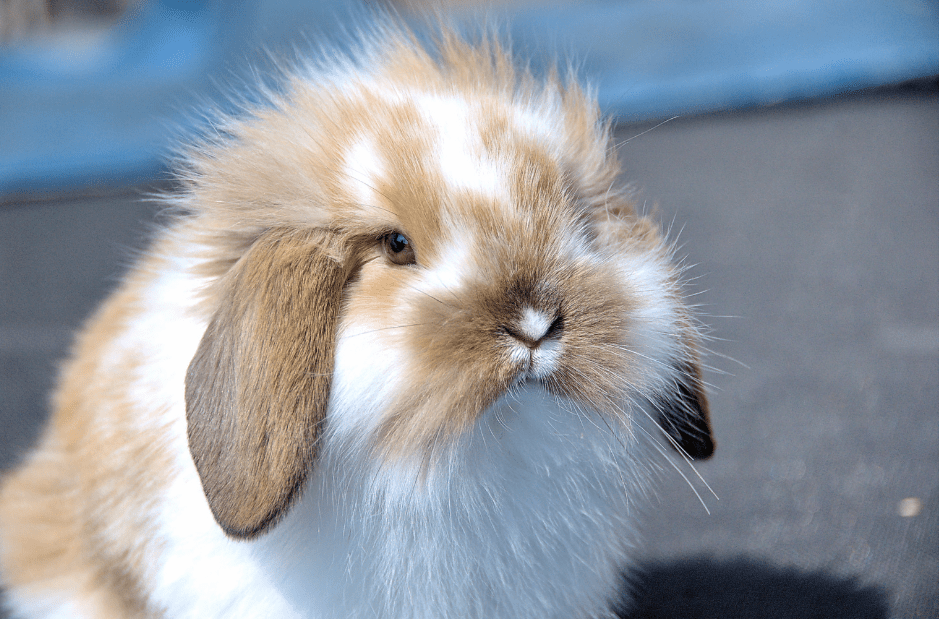
\includegraphics[width=\textwidth]{images/AFLBunny.png}
		%\caption{first figure}
	\end{minipage}\hfill
	\begin{minipage}{0.45\textwidth}
		\centering
		
\includegraphics[width=\textwidth]{images/AFLBunny++.png}
		%\caption{second figure}
	\end{minipage}
	\caption{On the left a young American Fuzzy Lop Rabbit used as the name for AFL and AFL++ and on the right AFL++'s logo. Images taken from \href{https://animalcorner.org/wp-content/uploads/2020/11/American-Fuzzy-Lop-Rabbit.png}{animalcorner.org} and AFL++'s \href{https://github.com/AFLplusplus/Website/blob/master/static/aflpp_bg.png}{website} respectively \cite{AFLBunny, AFLPlusPlusBunny}.}
	\label{fig:AFLbunny}
\end{figure}

As for the more popular fuzzers, American fuzzy lop\footnote{\url{https://github.com/google/AFL}} (AFL), which named after an American rabbit breed (see figure \ref{fig:AFLbunny}) and is a C and C++ focused mutation based gray box fuzzer released by Google. But due inactivity on Google's part the fork AFL++\footnote{\url{https://github.com/AFLplusplus/AFLplusplus}} has become more popular than the original and is maintained actively by the community \cite{27AFL++}. Not only is it actively maintained, but it is also actively used by researchers and the industry. Besides sparking the existence of AFL++, AFL has also triggered a python\footnote{\url{https://github.com/jwilk/python-afl}} focused version, a Ruby\footnote{\url{https://github.com/richo/afl-ruby}} focused one, a Go\footnote{\url{https://github.com/aflgo/aflgo}} focused version and is shown by Robert Heaton \cite{AFLWrapper} to not be difficult to write a wrapper for it.

A potential reason to the inactivity of Google on the AFL project could be the development of both Clusterfuzz\footnote{\url{https://google.github.io/clusterfuzz/}} and OSS-fuzz\footnote{\url{https://google.github.io/oss-fuzz/}}, a scalable fuzzing infrastructure and a combination of multiple fuzzers respectively. With the former one being used in OSS-fuzz as a back end to create a distributed execution environment. This with quite a bit of success,
\begin{quote} %note{currently at 44 700 issues, but the GitHub isn't updated yet}
	"As of May 2022, ClusterFuzz has found 29,000 bugs in Google (e.g. Chrome) and 36,000+ bugs in over 550 open source projects" and \newline
	"As of July 2022, OSS-Fuzz has found over 40,500 bugs in 650 open source projects."	
\end{quote} according to both the CusterFuzz and the OSS-Fuzz repository respectively \cite{31OSS-FuzzBugs}. 

Google is not the only one to come forward with a fuzzer. Even Microsoft has jumped on the bandwagon of fuzzing with its OneFuzz\footnote{\url{https://github.com/microsoft/onefuzz}}, a self-hosted Fuzzing-As-A-Service platform which is intended to be integrated with the CI/CD pipeline. Although looking at the given stars on the GitHub repository, it looks like Google's tools are more popular than Microsoft's ones. The last prominent fuzzer we will look at is the LibFuzzer\footnote{\url{https://llvm.org/docs/LibFuzzer.html}} made by LLVM, a generation based gray box fuzzer which is a part of the bigger LLVM project\footnote{\url{https://github.com/llvm/llvm-project/}} with the focus on the C ecosystem. Being in the same ecosystem as AFL, LibFuzzer can be used together with AFL and even share the same seed inputs.

\subsection{Testing CP and SMT with Fuzzers}
\label{fuzzing:testingWithFuzzers}
Until now we discussed fuzzers more generally, we would like to deliberate specific fuzzers build for testing constraint programming languages (CP) and satisfiability modulo theory (SMT) solvers.
\begin{figure}
	\centering
	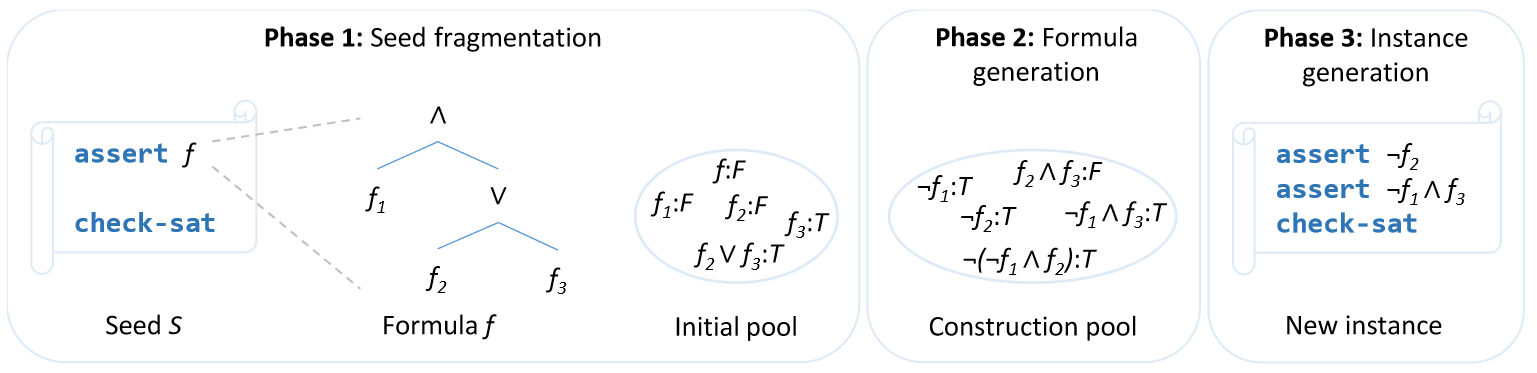
\includegraphics[width=1.0\textwidth]{images/STORM}
	\caption{Overview of the three STORM phases as presented by Muhammad Numair Mansur et al. in "Detecting Critical Bugs in SMT Solvers Using Blackbox Mutational Fuzzing" \cite{1mansur2020detecting}.}
	\label{fig:STORM}
\end{figure}
One of those fuzzers is STORM which is a mutation based black box fuzzer created by Muhammad Numair Mansur et al. \cite{1mansur2020detecting} to find critical bugs (i.e., wrongly sat or wrongly unsat) in SMT solvers. In their paper \cite{1mansur2020detecting} they explain the inner working thoroughly, but briefly summarized STORM creates an initial pool of smaller formulas from existing formulas found in seeds, uses another solver to create models of those smaller formulas. To then construct more complex formulas with the knowledge of their ground truth, with this STORM can test the SMT solver as represented in figure \ref{fig:STORM}. This novel way of fuzzing SMT solvers with inputs that are satisfiable by construction and has been cited significantly, considering that it is a recent paper.

\label{fuzzing:SemanticFusion}
Another technique for fuzzing SMT solvers is the one proposed by Dominik Winterer et al. with their fuzzer YinYang \cite{43YinYang}, which uses "Semantic Fusion" to test the solvers.
\begin{quote}
	\label{quote:Fuzzing:YinYang}
	"Our key idea is to fuse two existing equisatisfiable (i.e., both satisfiable or unsatisfiable) formulas into a new formula that combines the structures of its ancestors in a novel manner and preserves the satisfiability by construction. This fused formula is then used for validating SMT solvers."
	\newline
	-Dominik Winterer et al. in "Validating SMT Solvers via Semantic Fusion" \cite{43YinYang}.
\end{quote}
Dominik Winterer et al. take a free variable from each of the equisatisfiable formulas to be able to create a new variable using a reversible fusion function. For example, a formula \mbox{$\phi_1$ $\equiv$ X > 10} and \mbox{$\phi_2$ $\equiv$ Y < 9} with the fusion function for \mbox{Z = X + Y} would become \mbox{$\phi_3$ $\equiv$ (Z - Y) > 10 $\land$ (Z - X) < 9}, linking both satisfiable formulas together. For unsatisfiable formulas an extra conjunction is needed with the definition of the new variable, because a substitution could result in the loss of the unsatisfiability of the formula as mentioned in the paper \cite{43YinYang}. The results of the paper where also significant with 45 bugs in state-of-the-art SMT solvers in Z3\footnote{\url{https://github.com/Z3Prover/z3}} and CVC4\footnote{\url{https://github.com/CVC4/CVC4-archived}}. Dominik Winterer et al. also give multiple fusion functions such as multiplication and string concatenations which can be applied to integers and real numbers and strings respectively. Extending this technique to other data types or more fusion functions would not be difficult.


A last fuzzer we will discuss is Falcon, a fuzzer that extends the search space to also test the configuration of the SMT solvers. This fuzzer made by Peisen Yao et al. \cite{42FalconFuzzingConfigurationSettingsAndNormal} found quite the success by being the first to linking the configuration options to the operations and to then use this information to fuzz better.
When using STORM as the underlying fuzzer with the knowledge of the configuration space the authors managed to increase the code coverage by up to 18.8\%. When knowing that SMT solver such as Z3 and CVC4 contain more than 700,000 and 100,000 lines of code respectively means that any percentage is a significant number of extra lines covered.

\section{Types of bugs}
\label{fuzzing:TypesOfBugs}
Not only can we classify fuzzers, but we can also classify the types of bugs found by the fuzzers, as done in a recent paper \cite{1mansur2020detecting} by Muhammad Numair Mansur et al. being crashes, wrongly satisfied, wrongly unsatisfied or a hanging inputs. With some of these bugs being less acceptable than others. For example, as Muhammad Numair Mansur et al. describes, a crash is preferred for a constraint programming language (CP) over a wrongly unsatisfied model, since there is no way for the user to know that the solver failed in that last case (except for differentiation testing, more on that later). Meaning that the user will treat the result (wrongly) as correct, comparing this to a crash where it is clear that something went wrong is more transparent for the user. With hanging inputs, the user cannot draw incorrect conclusions and with wrongly satisfied models the user could check the model's instances and confirm the result before using it further. This is due to the fact that problems are frequently NP-hard meaning they are easy to confirm but hard to solve. 
For practical reasons we will be defining models that take more then 15 minutes to a timeout category and wrong amount of solutions to the critical bugs together with the wrongly satisfiable and wrongly unsatisfiable solution. We are aware that the types of bugs can be classified in even more detail, for example crashes into buffer overflows, invalid memory addressing and so on, but we choose to stay with a more general overview for now. An interesting classification to be added is the knowledge whether or not the bug is in the parser part of the PUT or not. The put could already fail on inputs during the interpretation of the inputs and as discussed, we would also like to detect bugs deeper in the PUT. As the authors of "Semantic Fuzzing with Zest" \cite{22SemanticFuzzing} would classify, is the bug in the syntactical or in the semantical part of the program?
%can use to \ref{intro:FussingSecurity}, but fitting it in this txt seems forced

\section{Other forms of testing}
\subsection{Differential testing}
\label{fuzzing:DifferentialTesting}
As mentioned above a lot of fuzzers use crashes to detect that the PUT has failed to provide a correct output or when possible, use differential testing. This latter one uses a single or multiple analog programs to test if the PUT gave the same output as the analog programs. As Christian Klinger et al. did in their paper \cite{48klinger2019differentially} by applying "bugs-as-deviant-behavior" they try to find precision and soundness mistakes with input creation via seed files to compare the output to similar programs. 
Unfortunately, neither crash based nor differential testing is ideal, crash based fuzzing will not trigger on wrong outputs and differential testing requires that one or multiple analog programs exits preferably with a different implementation to reduce overlapping bugs. The latter technique may therefore not always be possible due to the existence of those analog programs.

\subsection{Metamorphic testing}
\label{fuzzing:MetamorphicTesting}
In situations where the existence of analog programs would be a limited factor metamorphic testing could be a solution. A nicely worded definition would be 

\begin{quote}
	\label{quote:MetaMorphic}
	"Metamorphic testing (...) involves generating new test cases from existing ones, where the expected result of a new test case can be generated from the result of an existing test via a metamorphic relation. By comparing the results of the
	original test with the new one we can identify cases where the metamorphic relations are broken (...)".
	\newline
	-\"{O}zg\"{u}r Akg\"{u}n et al. in "Metamorphic Testing of Constraint Solvers" \cite{50akgun2018metamorphic}.
\end{quote}

\noindent This technique uses knowledge of the domain to tell if subsequent solutions may be wrong. For example, in "TestMC: Testing Model Counters using Differential and Metamorphic Testing" \cite{49usman2020testmc} the authors add an extra restriction to a variable in a formula to test if the number of models reduces (or remains equal). Or when given an equivalent formula that the number of models remain the same compared to the original. This technique no longer depends on a secondary oracle but does depend on multiple executions and could miss a bug that occurs in multiple situations. This technique has been applied in combination with differential testing to test constraint solvers with success by Akg{\"u}n, {\"O}zg{\"u}r et al. \cite{50akgun2018metamorphic}. In which they express how well this technique fits with testing constraint solving, due to the availability of metamorphic transformations.

\section{The oracle problem}
\label{fuzzing:OracleProblem}
The oracle problem describes the issue of telling if a PUTs output was, given the input, correct or not. As expressed in "The Oracle Problem in Software Testing: A Survey": 
\begin{quote}
	"Given an input for a system, the challenge of distinguishing the corresponding desired, correct behavior from potentially incorrect behavior is called the test oracle problem."
	\newline
	-Earl T. Barr et al. in "The Oracle Problem in Software Testing: A Survey" \cite{10barr2014oracleProblem}.
\end{quote}
In their paper they discuss four categories specified test oracles, derived test oracles, implicit test oracles and the absence of test oracles. The biggest category would be the specified test oracles which contains all the possible encoding of specifications like modeling languages UML, Event-B and more. Their derived test oracles classification contains all forms of knowledge obtained from documentation on how the program should work or by knowledge of previous versions of the program. The last two oracles' categories come down to the use of knowing that crashes are always unwanted and the human oracle such as crowdsourcing respectively.

\subsection{Handling the oracle problem}
\label{fuzzing:handelingOracelproblem}
Although the approach of by Bugariu and M\"uller in "Automatically testing string solvers" \cite{9bugariu2020automaticallyTestingStringSolvers} falls in the first category being, a black box fuzzer, their approach is innovative. While most fuzzers either use crashes or differential testing (more on that later) to find bugs, they know the (un)satisfiability of their formulas by the way of they are constructed. For satisfiable formulas they generate trivial formulas and then by satisfiability preserving transformations increase the complexity and for unsatisfiable formulas they use \mbox{$\neg$ A $\land$ A'}, with A' being an equivalent formula but different formula for A, to create the trivial unsatisfiable formulas. To increase the complexity of those trivial formulas, they again depend on satisfiability preserving transformation. This technique of creating formulas satisfiable by construction has also been applied to SMT solvers by Muhammad Numair Mansur et al. called STORM \cite{1mansur2020detecting} which uses mutational input creation compared to the previous generation based techniques. In the paper the authors dissect all SMT assertions into their sub-formulas and create an initial pool. In this pool the sub-formulas are checked if they satisfy or not and with this knowledge new formulas are created for the population pool with ground truth, from this pool new theories are created and tested. This makes that STORM does not need an oracle to test the entire theory, but only the smaller sub-formulas.


%somewhere a ref to later chapter input simplification (minimisation differantioation)
\section{Opinions against Fuzzing}
\label{fuzzing:OpinionsAgainstFuzzing}
We have talked about the successes of fuzzing, but there are also voices against fuzzing. As William M. McKeeman \cite{39differentialTesting} writes some developers do not like the automatic way of adding more bugs to their backlog and see it as unreasonable. "Why would a person do this (obscure actions)?" and that fuzzing seems to generate an infinite number of bugs are also pet peeves of developers according to McKeeman.
Although we have a bias due to writing this thesis about fuzzing, we think that those perspectives should be acknowledged in this paper. Although, this is not a single view shared by all developers from the papers \cite{43YinYang, 42FalconFuzzingConfigurationSettingsAndNormal, 47zhang2019finding} and others we see a positive response to newly found bugs by the respective developers. Some have even started implementing fuzzers \cite{44Stringfuzz} in their toolchain to detect bugs.

\section{Conclusion}
\label{fuzzing:conclusion}
In this chapter we have seen an overview of what fuzzers are, which are used in the industry and how they work. We have seen techniques and fuzzer specified for SMT solver but also for constraint solvers. To finally end with some problems around getting the difference between correct and incorrect behavior and a small paragraph on the perspective of the developers on fuzzing.

%%% Local Variables: 
%%% mode: latex
%%% TeX-master: "thesis"
%%% End: 
